\documentclass[a4paper]{article}
\usepackage[utf8]{inputenc}
\usepackage{graphicx} % Required for including images
\usepackage[font=small,labelfont=bf]{caption}
\usepackage{courier}
\usepackage{amsmath}
\usepackage{color}
\usepackage{listings}
\usepackage{subcaption}
\usepackage{booktabs}
\usepackage[table,xcdraw]{xcolor}

\usepackage{array}
\newcolumntype{M}[1]{>{\centering\arraybackslash}m{#1}}

\lstset{
    basicstyle=\ttfamily,
    language=Octave,
    morecomment = [l][\itshape\color{blue}]{\%}
}

\addtolength{\oddsidemargin}{-.875in}
\addtolength{\evensidemargin}{-.875in}
\addtolength{\textwidth}{1.75in}

\addtolength{\topmargin}{-.875in}
\addtolength{\textheight}{1.75in}

\setlength{\parindent}{0pt}
\setlength{\parskip}{0.5em}

\renewcommand{\figurename}{Figura}
\renewcommand{\tablename}{Tabla}

\newcommand{\bold}[1]{\textbf{\texttt{#1}}}
\newcommand{\italic}[1]{\textit{\texttt{#1}}}

\newcommand{\reffig}[1]{\textbf{Figura \ref{#1}}}
\newcommand{\reftable}[1]{\textbf{Tabla \ref{#1}}}

\title{TP 2: Algoritmos de Clasificación Supervisada}
\author{Giuliano Scaglioni}
\date{Septiembre 2019}

\begin{document}

\clearpage\maketitle
\thispagestyle{empty}

\newpage

\setcounter{page}{1}

\section{Deportes en el río}
  \subsection{Implementación}
  La implementación del programa se realizó en Go utilizando el algoritmo ID3 para construir el árbol de decision.

  \subsubsection{Entidades}
    En la implementación se definieron las siguientes entidades
    \begin{itemize}
      \item \bold{Classifier}: es una abstracción de un clasificador. Define una interfaz que permite clasificar un ejemplo. Cada clasificador implementado en el trabajo práctico, implementa esta interfaz.
      \item \bold{Metric}: es un tipo que almacena metricas de evaluación de un clasificador. Además provee metodos para evaluar un clasificador independientemente de su implementación.
      \item \bold{Example}: representa un ejemplo, su implementación es un mapa donde cada entrada tiene como clave el nombre del atributo y como valor, el valor que tiene ese atributo en el ejemplo.
      \item \bold{DecisionTree}: representa un árbol de decisión, para crear uno, se pasa una lista de ejemplos y el nombre del atributo objetivo. La implementación interna de esta entidad utiliza el algoritmo ID3 para crearlo. En la creación de un árbol de decisión, a su vez, se utilizan otras entidades, estas son:
      \begin{itemize}
        \item \bold{Node}: representa un nodo del arbol de decisión y define comportamiento para obtener el tipo de nodo, obtener la lista de hijos de este, agregar hijos, entre otros métodos necesarios para su representación.
        \item \bold{AttrNode}: es una implementación de Node para los nodos que representan un atributo.
        \item \bold{ValNode}: es una implementación de Node para los nodos que representan los valores posibles de un atributo.
        \item \bold{ClassNode}: es una implementación de Node para los nodos que representan una clase. Esta implementación no permite agregar hijos pues este tipo de nodos siempre es hoja.
      \end{itemize}
    \end{itemize}
  \subsubsection{Visualización del árbol}
    El programa implementado construye el árbol a partir de una lista de examples y el atributo a predecir, y genera como salida el árbol en formato Graphviz dot. 

    Además se provee una utilidad implementada en Vue.js que permite crear el árbol a partir de un archivo csv y visualizar el árbol de decisión desde el navegador utilizando como backend el programa implementado.
\subsection{Árboles de decisión}
Se utilizó el programa descripto anteriormente para construír el árbol de decisión para el conjunto de datos provisto.

\begin{figure}[h]
  \centering
    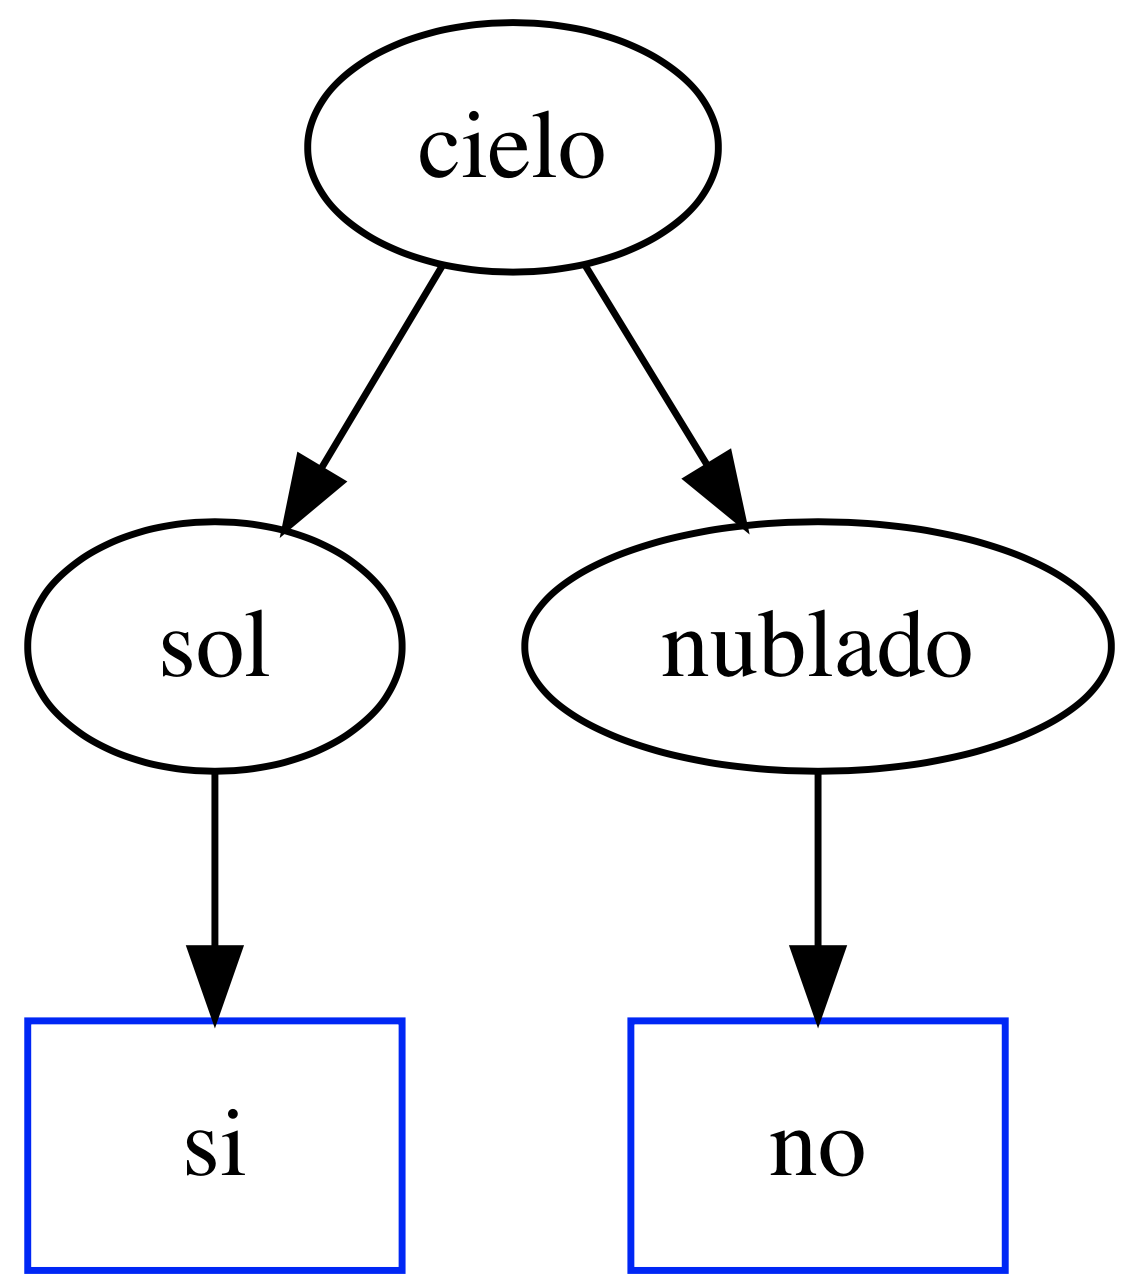
\includegraphics[scale=0.2]{img/tree1.png}
  \caption{Árbol de decisión construído.}
  \label{ej1-tree1}
\end{figure}

Como se puede observar en la \reffig{ej1-tree1}, el único atributo relevante para determinar si la persona disfruta de deportes en el río es el cielo. Si se observa la table, se puede ver que ademas del cielo, tambien la temperatura determina si disfruta o no. En la implementación del algoritmo \bold{ID3} se decidió que, en casos de empte, se conserve el primer atributo evaluado, en este caso, cielo.

Si se compara con los datos de la \reftable{tab:dataset-1}, se puede ver que coincide en que, para determinar si disfruta, el atributo cielo tiene que tener el valor sol.

\begin{table}[h]
  \centering
  \begin{tabular}{ccccccc}
  Cielo                          & Tempe. & Humedad & Viento & Agua   & Pronós.    & ¿Disfruta?                \\ \hline
  {\color[HTML]{009901} sol}     & calida & normal  & fuerte & calida & estable   & {\color[HTML]{009901} si} \\
  {\color[HTML]{009901} sol}     & calida & alta    & fuerte & calida & estable   & {\color[HTML]{009901} si} \\
  {\color[HTML]{CB0000} nublado} & frio   & alta    & fuerte & calida & cambiante & {\color[HTML]{CB0000} no} \\
  {\color[HTML]{009901} sol}     & cálida & alta    & fuerte & fria   & cambiante & {\color[HTML]{009901} si}
  \end{tabular}
  \caption{Conjunto de datos provisto}
  \label{tab:dataset-1}
  \end{table}

Al agregar el nuevo ejemplo indicado se obtuvo el árbol de decisión de la \reffig{ej1-tree2}.

\begin{figure}[h]
  \centering
    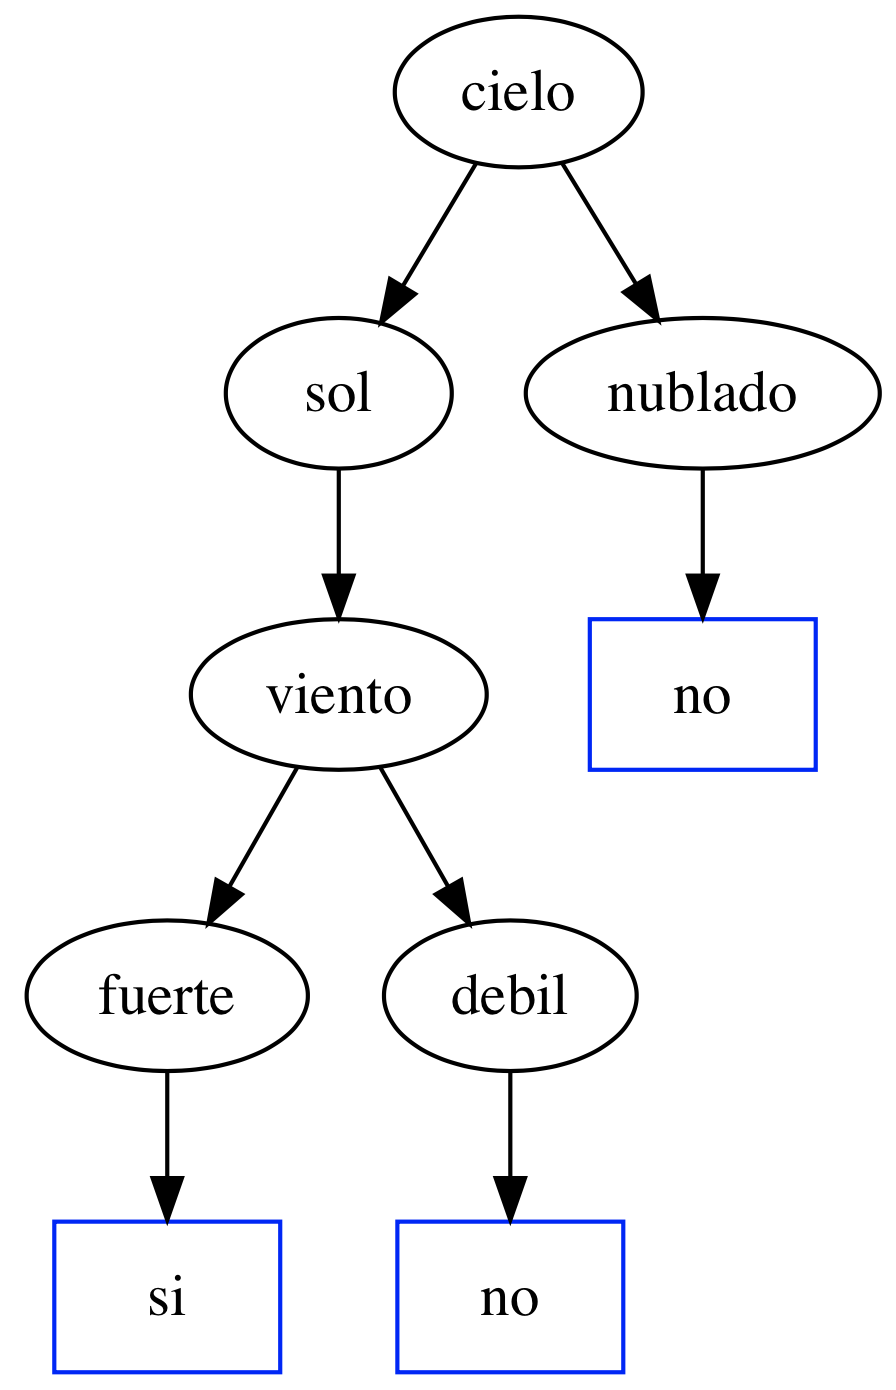
\includegraphics[scale=0.4]{img/tree2.png}
  \caption{Árbol de decisión construído.}
  \label{ej1-tree2}
\end{figure}

Como se puede observar en la \reftable{tab:dataset-2}, en caso de que el atributo cielo sea sol tambien se debe comprobar el valor del atributo viento para determinar si disfruta, lo cual coincide con el árbol de decisión obtenido.

\begin{table}[h]
  \centering
  \begin{tabular}{ccccccc}
  Cielo                          & Tempe. & Humedad & Viento                        & Agua   & Pronós.    & ¿Disfruta?                \\ \hline
  {\color[HTML]{009901} sol}     & calida & normal  & {\color[HTML]{009901} fuerte} & calida & estable   & {\color[HTML]{009901} si} \\
  {\color[HTML]{009901} sol}     & calida & alta    & \color[HTML]{009901} fuerte  & calida & estable   & {\color[HTML]{009901} si} \\
  {\color[HTML]{CB0000} nublado} & frio   & alta    & fuerte                        & calida & cambiante & {\color[HTML]{CB0000} no} \\
  {\color[HTML]{009901} sol}     & calida & alta    & \color[HTML]{009901} fuerte & fria   & cambiante & {\color[HTML]{009901} si} \\
  {\color[HTML]{009901} sol}     & calida & normal  & {\color[HTML]{CB0000} debil}  & calida & estable   & {\color[HTML]{CB0000} no}
  \end{tabular}
  \caption{Conjunto de datos con el ejemplo agregado}
  \label{tab:dataset-2}
  \end{table}

\newpage
\section{Titanic}

\subsection{Acondicionamiento del dataset}
El conjunto de datos fue modificado eliminando los atributos no relevantes para la clasificación de pasajeros, como el ID del pasajero, el numero de ticket, etc. Además, los atributos edad y tarifa, fueron discretizados.

El dataset final utilizado se encuentra dentro de la carpeta \italic{datasets} en el repositorio de código bajo el nombre \italic{titanic-discretized.csv}. 

\subsection{Conjuntos de prueba y entrenamiento}
Para obtener los conjuntos de prueba y entrenamiento, se implementó un programa que permite dividir un dataset aleatoriamente indicando el porcentaje de test que se requiere. Este programa esta bajo el nombre \italic{cmd/splitset} en el repositorio de código.

Para determinar el porcentaje de test a utilizar, se realizaron 5 divisiones aleatorias distintas para test sets de 20\%, 25\%, 30\% y 35\% del conjunto de datos total. Para cada porcentaje se obtuvo la varianza y el promedio de la precisión obtenida a partir de la evaluacion de los distintos clasificadores con cada training/test set. En la \reftable{tab:testset-summary} se sumarizan los resultados obtenidos.

\begin{table}[h]
  \centering
  \begin{tabular}{@{}cllllllll@{}}
  \toprule
  \multicolumn{1}{l}{}       & \multicolumn{2}{l}{Entropía de Shannon} & \multicolumn{2}{l}{Índice de Gini} & \multicolumn{2}{l}{R. Forest - Shannon} & \multicolumn{2}{l}{R. Forest - Gini} \\ \midrule
  \multicolumn{1}{l}{Tamaño} & Varianza           & Promedio           & Varianza         & Promedio        & Varianza           & Promedio           & Varianza          & Promedio         \\
  20\%                       & 0.080              & 0.800              & 0.062            & 0.820           & 0.062              & 0.820              & 0.062             & 0.820            \\
  25\%                       & 0.024              & 0.839              & 0.024            & 0.839           & 0.024              & 0.839              & 0.024             & 0.839            \\
  30\%                       & 0.014              & 0.701              & 0.014            & 0.701           & 0.014              & 0.701              & 0.014             & 0.701            \\
  35\%                       & 0.006              & 0.596              & 0.014            & 0.640           & 0.008              & 0.610              & 0.014             & 0.640            \\ \bottomrule
  \end{tabular}
  \caption{Valores de varianza y promedio de la precisión en funcion del tamaño del conjunto de prueba}
  \label{tab:testset-summary}
  \end{table}

  \begin{figure}[h]
    \centering
    \begin{subfigure}{.4\textwidth}
      \centering
      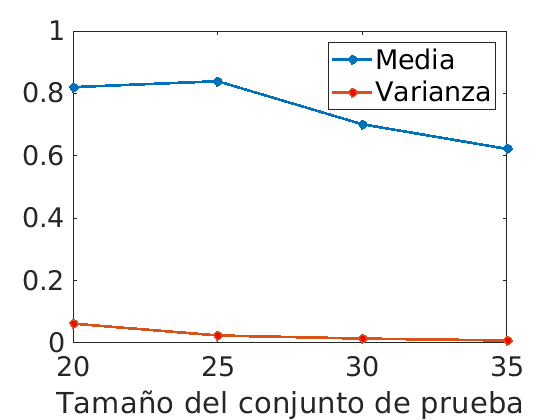
\includegraphics[width=\linewidth]{img/test-set-shannon.png}
      \caption{Entropía de Shannon}
      \label{test-size:sfig1}
    \end{subfigure}%
    \begin{subfigure}{.4\textwidth}
      \centering
      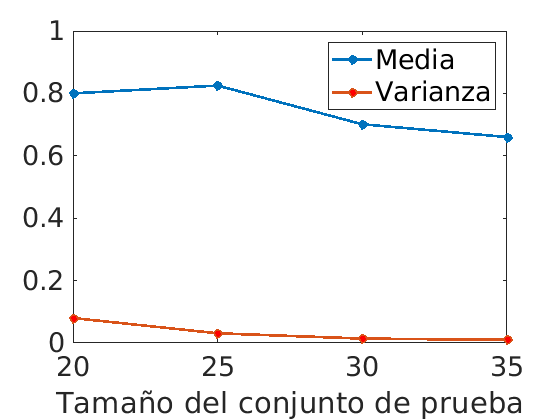
\includegraphics[width=\linewidth]{img/test-set-gini.png}
      \caption{Índice de Gini}
      \label{test-size:sfig2}
    \end{subfigure}
    \begin{subfigure}{.4\textwidth}
      \centering
      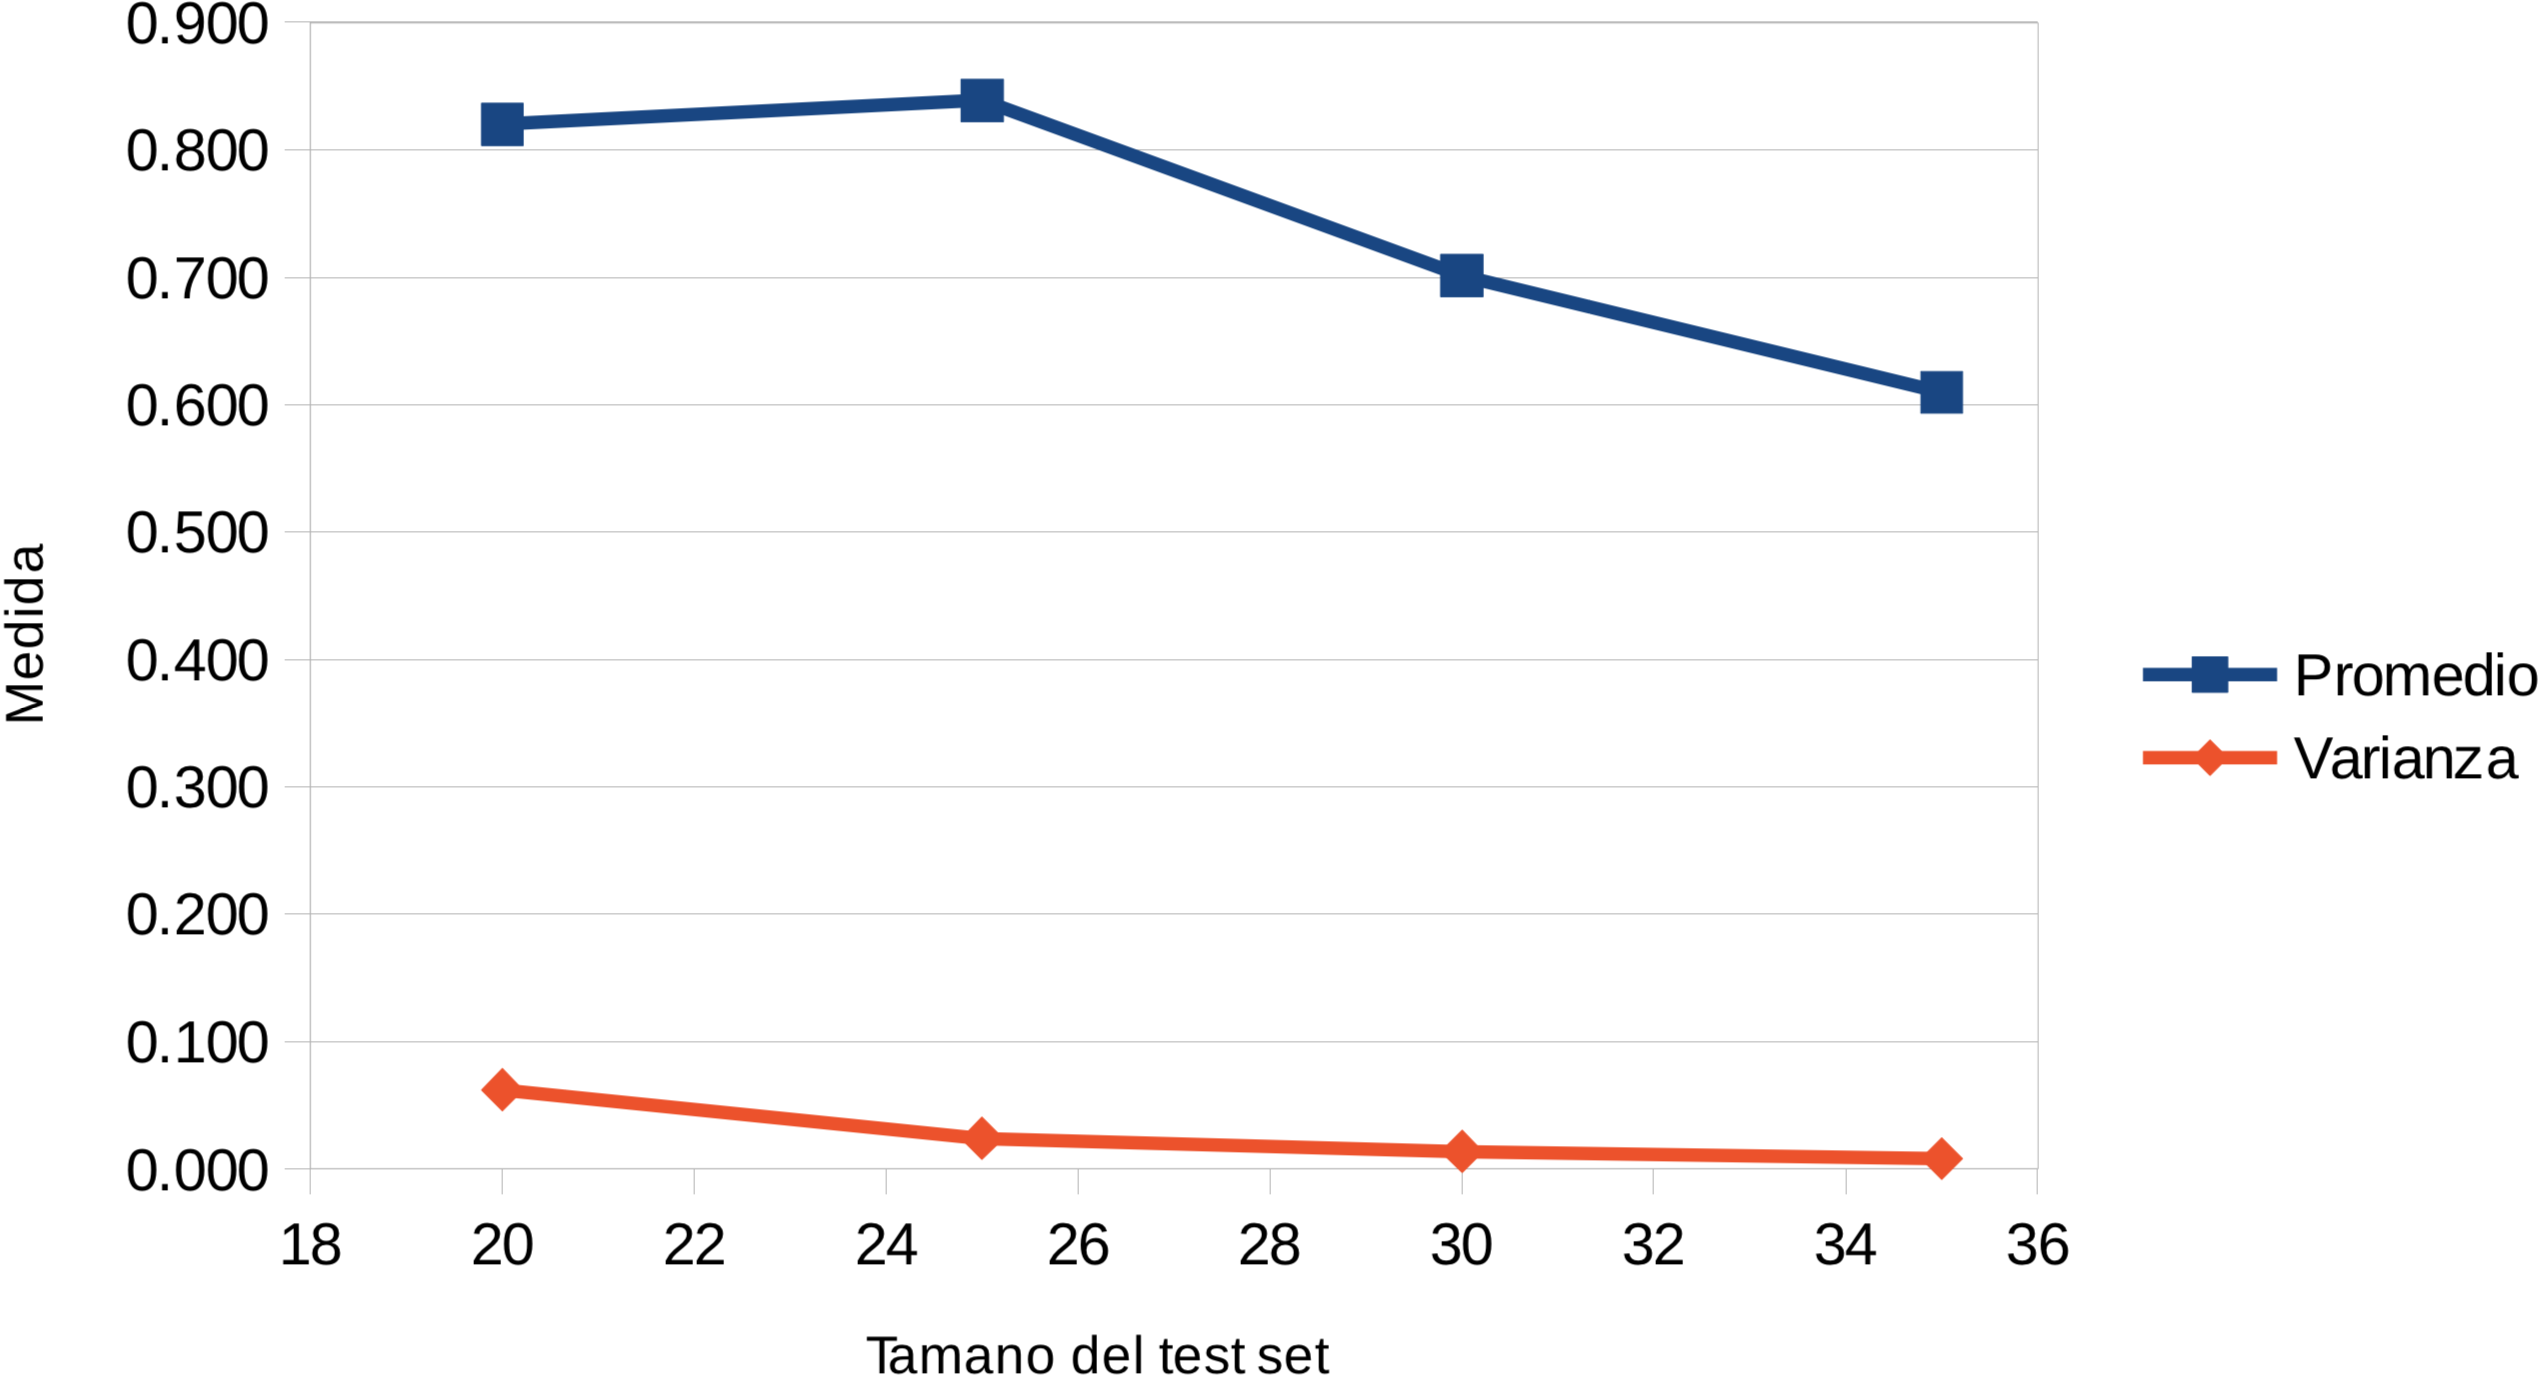
\includegraphics[width=\linewidth]{img/test-set-rf-shannon.png}
      \caption{Random Forest con Entropía de Shannon}
      \label{test-size:sfig3}
    \end{subfigure}
    \begin{subfigure}{.4\textwidth}
      \centering
      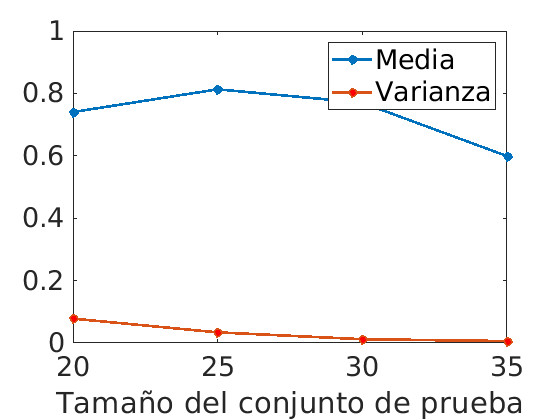
\includegraphics[width=\linewidth]{img/test-set-rf-gini.png}
      \caption{Random Forest con Índice de Gini}
      \label{test-size:sfig4}
    \end{subfigure}
    \caption{Gráficos de la varianza y promedio de la precisión en funcion del tamaño del test set}
    \label{test-size:fig}
  \end{figure}

  Como se puede observar en la \reffig{test-size:fig}, 25\% de test set es el valor que provee una varianza en los resultados reducida sin comprometer la precisión obtenida. Por esta razón, la división elegida para utilizar en los próximos ejercicios es de 75\% para training y 25\% para test.

  \subsection{Matrices de confusion}
  Para obtener las matrices de confusion, se dividieron los datos en un conjunto de prueba y otro de entrenamiento. Se entreno cada clasificador con el mismo conjunto de entrenamiento y se realizaron todas las evaluaciones con le mismo conjunto de prueba.
  
  En todos los casos se podo el arbol utilizando la condicion de que cada nodo raiz debia tener al menos el 10\% del tamano del conjunto de entrenamiento. Las evaluaciones del metodo Random Forest se realizaron con 10 arboles en cada clasificador.

  Las matrices de confusion obtenidas para cada evaluacion se pueden ver en la \reffig{titanic-cm:fig}.

  \begin{figure}[h]
    \centering
    \begin{subfigure}{.4\textwidth}
      \centering
      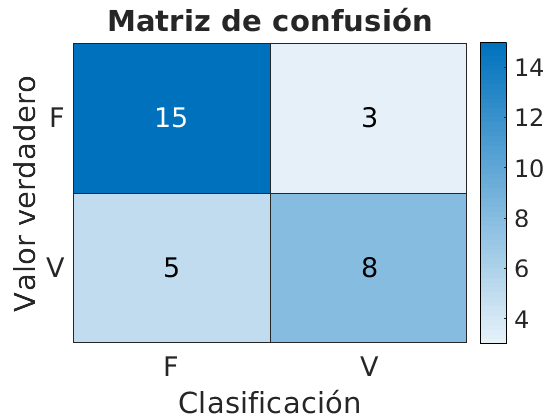
\includegraphics[width=\linewidth]{img/cm-shannon.png}
      \caption{Entropía de Shannon}
      \label{titanic-cm:sfig1}
    \end{subfigure}%
    \begin{subfigure}{.4\textwidth}
      \centering
      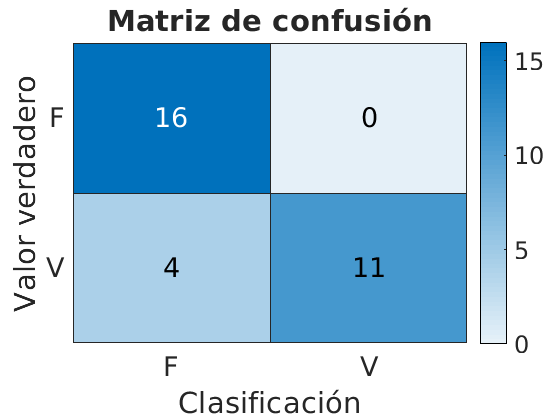
\includegraphics[width=\linewidth]{img/cm-gini.png}
      \caption{Índice de Gini}
      \label{titanic-cm:sfig2}
    \end{subfigure}
    \begin{subfigure}{.4\textwidth}
      \centering
      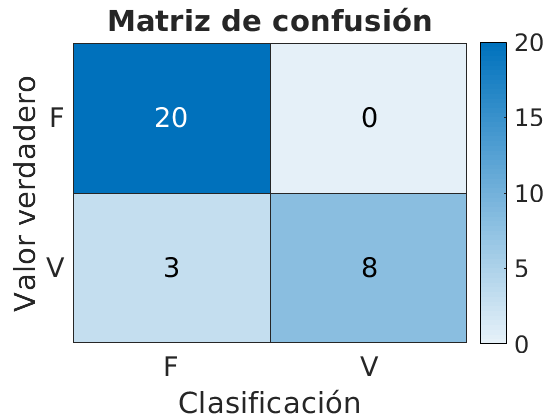
\includegraphics[width=\linewidth]{img/cm-rf-shannon.png}
      \caption{Random Forest con Entropía de Shannon}
      \label{titanic-cm:sfig3}
    \end{subfigure}
    \begin{subfigure}{.4\textwidth}
      \centering
      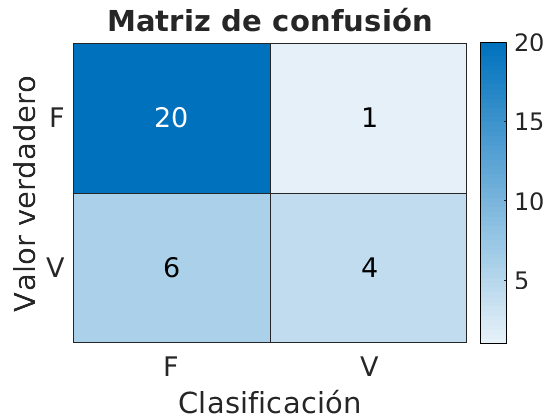
\includegraphics[width=\linewidth]{img/cm-rf-gini.png}
      \caption{Random Forest con Índice de Gini}
      \label{titanic-cm:sfig4}
    \end{subfigure}
    \caption{Matrices de confusion de cada evaluacion}
    \label{titanic-cm:fig}
  \end{figure}

\subsection{Precision vs. cantidad de nodos}

\newpage

\section{Opiniones de usuarios}

\subsection{Comentarios con una estrella}
Se implemento un programa que calcula la cantidad de palabras promedio que tienen los comentarios de una estrella. El mismo puede encontrarse bajo \bold{cmd/reviewswordcount} en el repositorio de codigo.

Al correrlo con el conjunto de datos provisto, el resultado es que los comentarios con una estrella tienen en promedio $12.22$ palabras.

\subsection{Conjunto de entrenamiento}
Se dividieron los datos en un conjunto de entrenamiento y otro de prueba con 70\% y 30\% de los datos respectivamente de forma aleatoria con el programa \bold{splitset} comentado en el ejercicio anterior.

Se eliminaron los atributos que no eran numericos dejando solo \textit{wordCount}, \textit{sentimentValue} y \textit{titleSentiment} conviertiendo este ultimo a -1 para los negativos y 1 para los positivos.

Luego se analizo el conjunto de entrenamiento para ver como se distribuian los ejemplos en el espacio, con el objetivo de proponer una funcion distancia efectiva.

\begin{figure}[h]
  \centering
    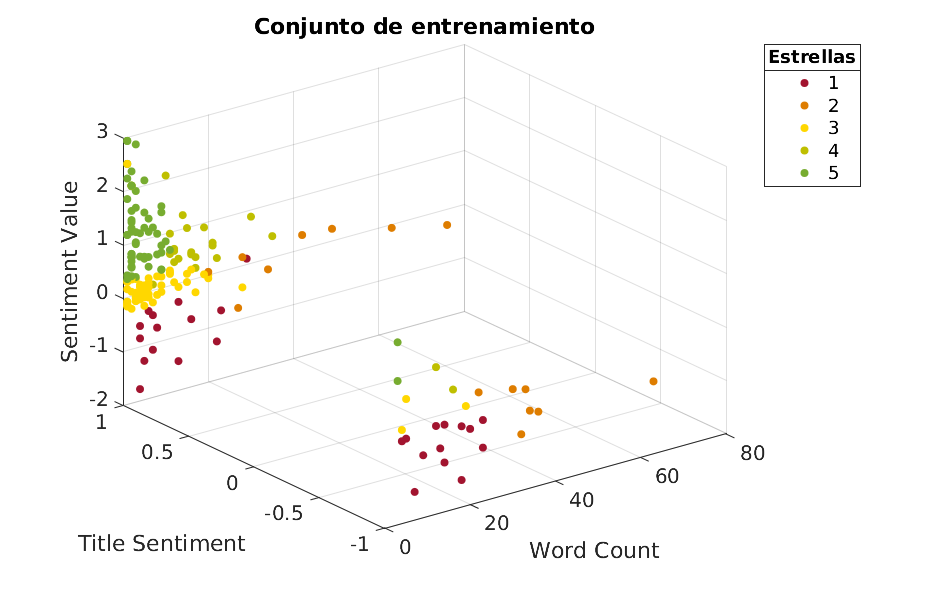
\includegraphics[scale=0.5]{img/knn-training-set-scatter.png}
  \caption{Grafico de dispersion de los ejemplos del conjunto de entrenamiento}
  \label{fig:ej3-scatter-training}
\end{figure}


\subsection{Funcion distancia}
Como se puede observar en la \reffig{fig:ej3-scatter-training}, la dimension WordCount no aporta una separacion significativa entre clases. Se puede ver que predominan algunos puntos naranjas (comentarios de dos estrellas) en la region donde mas palabras hay, pero la mayor parte de los puntos se encuentran en los valores bajos. Por otro lado, se distingue que Sentiment Value si separa los puntos entre clases de forma marcada entre las clases de 1, 3 y 5 estrellas. Finalmente, Title Sentiment aporta una separacion pero menos marcada, trayendo al plano TitleSentiment -1 mayor cantidad de puntos rojos.

Por la razones explicadas, se decidio dar mayor relevancia a Sentiment Value, luego a Title Sentiment y por ultimo a Word Count, proponiendo la funcion distancia siguiente:

\begin{equation}
  d(\vec{x},\vec{y}) = \left \|(\vec{x}-\vec{y})\begin{pmatrix}
    1 & 0 & 0\\ 
    0 & 2 & 0\\ 
    0 & 0 & 3
    \end{pmatrix}\right \|
\end{equation}

Donde $\vec{x}$ e $\vec{y}$ son ejemplos cuya primer componente es el Word Count, la segunda el Title Sentiment y la tercera el Sentiment Value.

\end{document}